\documentclass[12pt,letterpaper]{hmcpset}
\usepackage[margin=1in]{geometry}
\usepackage{graphicx}
\usepackage{url}
\usepackage{enumitem}

% info for header block in upper right hand corner
\name{ }
\class{Math 65}
\assignment{HW 8}
\duedate{Thursday, May 26, 2016}

\newcommand{\pn}[1]{\left( #1 \right)}
\newcommand{\abs}[1]{\left| #1 \right|}
\newcommand{\bk}[1]{\left[ #1 \right]}

\newcommand{\RR}{\mathbb{R}}
\newcommand{\m}[1]{\begin{bmatrix} #1 \end{bmatrix}}
\newcommand{\ind}{\leavevmode{\parindent=1em\indent}}

\renewcommand{\labelenumi}{{(\alph{enumi})}}

\begin{document}

\problemlist{1, 2, 3, 4, 5}

\begin{problem}[1]
    For each linear system of DEs given below,
    \begin{enumerate}[label=(\roman*)]
        \item Classify the origin as a saddle, center, spiral,
            deficient node, improper node or star node,
        \item Identify it as neutrally stable, unstable or
            asymptotically stable (you may refer to Tables 6.5.1 and
            6.5.2 in Borrelli \& Coleman, which is available as a
            handout on our Sakai site),
        \item Sketch the orbital portrait for each system. You may use
            ODEToolkit (\url{http://odetoolkit.hmc.edu}), Mathematica, or some
            other program to help you, but you should try to see if you can draw
            it yourself first without hints from the computer.
    \end{enumerate}
    \begin{enumerate}
        \item $\begin{cases}
            x'&\hspace{-.1in}=4y\\
            y'&\hspace{-.1in}=-x\end{cases}$\\ 
            Eigenvalues are $\lambda_1=2i$, $\lambda_2=-2i$ with
            corresponding eigenvectors $\mathbf{v}_1=\m{2\\i}$,
            $\mathbf{v}_2=\m{2\\-i}$.
        \item $\begin{cases}
            x'&\hspace{-.1in}=-x-4y\\
            y'&\hspace{-.1in}=x-y\end{cases}$\\\\
            Eigenvalues are $\lambda_1=-1+2i$, $\lambda_2=-1-2i$ with
            corresponding eigenvectors $\mathbf{v}_1=\m{2\\-i}$,
            $\mathbf{v}_2=\m{2\\i}$.
        \item $\begin{cases}
            x'&\hspace{-.1in}=2x+y\\
            y'&\hspace{-.1in}=-x+4y\end{cases}$\\\\ 
            Eigenvalues are $\lambda_1=\lambda_2=3$ with corresponding
            eigenspace spanned by the eigenvector
            $\mathbf{v}_1=\m{1\\1}$. Hence the eigenspace is
            deficient. A generalized eigenvector is
            $\mathbf{v}_2=\m{0\\1}$.
    \end{enumerate}
\end{problem}
\begin{problem}[1 cont.]
    \begin{enumerate}
        \setcounter{enumi}{3}
        \item $\begin{cases}
            x'&\hspace{-.1in}=x-2y\\
            y'&\hspace{-.1in}=x+4y\end{cases}$\\
            Eigenvalues are $\lambda_1=3$, $\lambda_2=2$ with
            corresponding eigenvectors $\mathbf{v}_1=\m{1\\-1}$,
            $\mathbf{v}_2=\m{2\\-1}$.
    \end{enumerate}
\end{problem}
\begin{solution}
    \vfill
\end{solution}
\newpage

\begin{problem}[2]
    \begin{enumerate}
        \item Consider a $2\times2$ system of first-order linear,
            constant-coefficient, homogeneous differential equations
            where the system matrix $A$ is real and has \textit{exactly
            one zero eigenvalue}. Write the general form for the set
            of solutions to any such system.
        \item Sketch orbital portraits for the various distinct cases
            where exactly one eigenvalue is $0$. Explain why your
            gallery of portraits represents all the possible cases.
\end{enumerate}
\end{problem}
\begin{solution}
    \vfill
\end{solution}
\newpage

\begin{problem}[3]
    Write down a system of linear, homogeneous, first-order,
    constant-coefficient differential equations that could support the
    following graph.  The straight trajectories (and their
    orientations) are the only ones that you must preserve.  The large
    arrows are just meant to show the general trend of the
    trajectories in the rest of the phase plane.  Also, use ODEToolkit
    or Mathematica or some other computer program to draw some
    solution trajectories for your differential equations to show that
    they match the diagram below.
    \begin{center}
        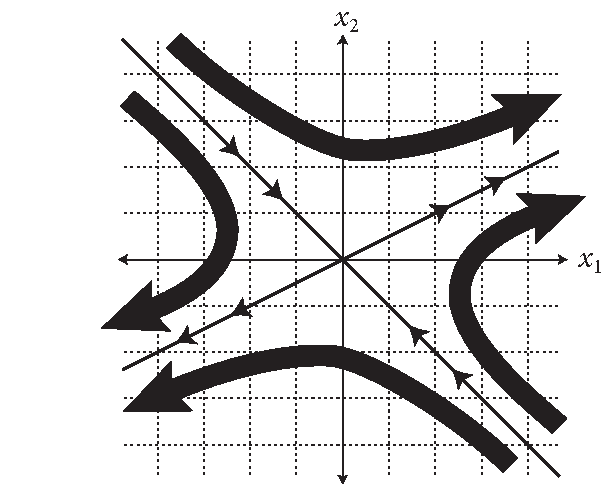
\includegraphics[scale=0.8]{img/may_26_3}
    \end{center}
\end{problem}
\begin{solution}
    \vfill
\end{solution}
\newpage

\begin{problem}[4]
    Consider the system of differential equations
    \[
        \mathbf{x}'(t)=\m{-1&2\\-6&-9}\mathbf{x}+\m{7\\21}.
    \]
    \begin{enumerate}
        \item Find the equilibrium point for this system of
            differential equations.  In other words, find values for
            $x_1$ and $x_2$ such that $x_1'=0$ and $x_2'=0$.  Let those
            values of $x_1$ and $x_2$ be denoted as $a$ and $b$.
        \item Let $u_1(t)=x_1(t)-a$ and $u_2(t)=x_2(t)-b$.  What new
            system of differential equations results for $u_1$ and
            $u_2$?  Solve it by hand using your favorite method.
        \item Find the solution to the original system of equations
            for the initial condition $x_1(0)=3$ and $x_2(0)=-1$. What
            is the behavior of your solution as $t\to\infty$?  How could
            you have predicted that long-term behavior simply based on
            the eigenvalues of the matrix alone?
    \end{enumerate}
\end{problem}
\begin{solution}
    \vfill
\end{solution}
\newpage

\begin{problem}[5]
    Here is a simplified diagram of a car. The suspension at each axle
    (springs, tires, and shock absorbers) is modeled by a spring and
    damper. Only a spring is shown in the figure below, but assume
    that there is some damping there too.
    \begin{center}
        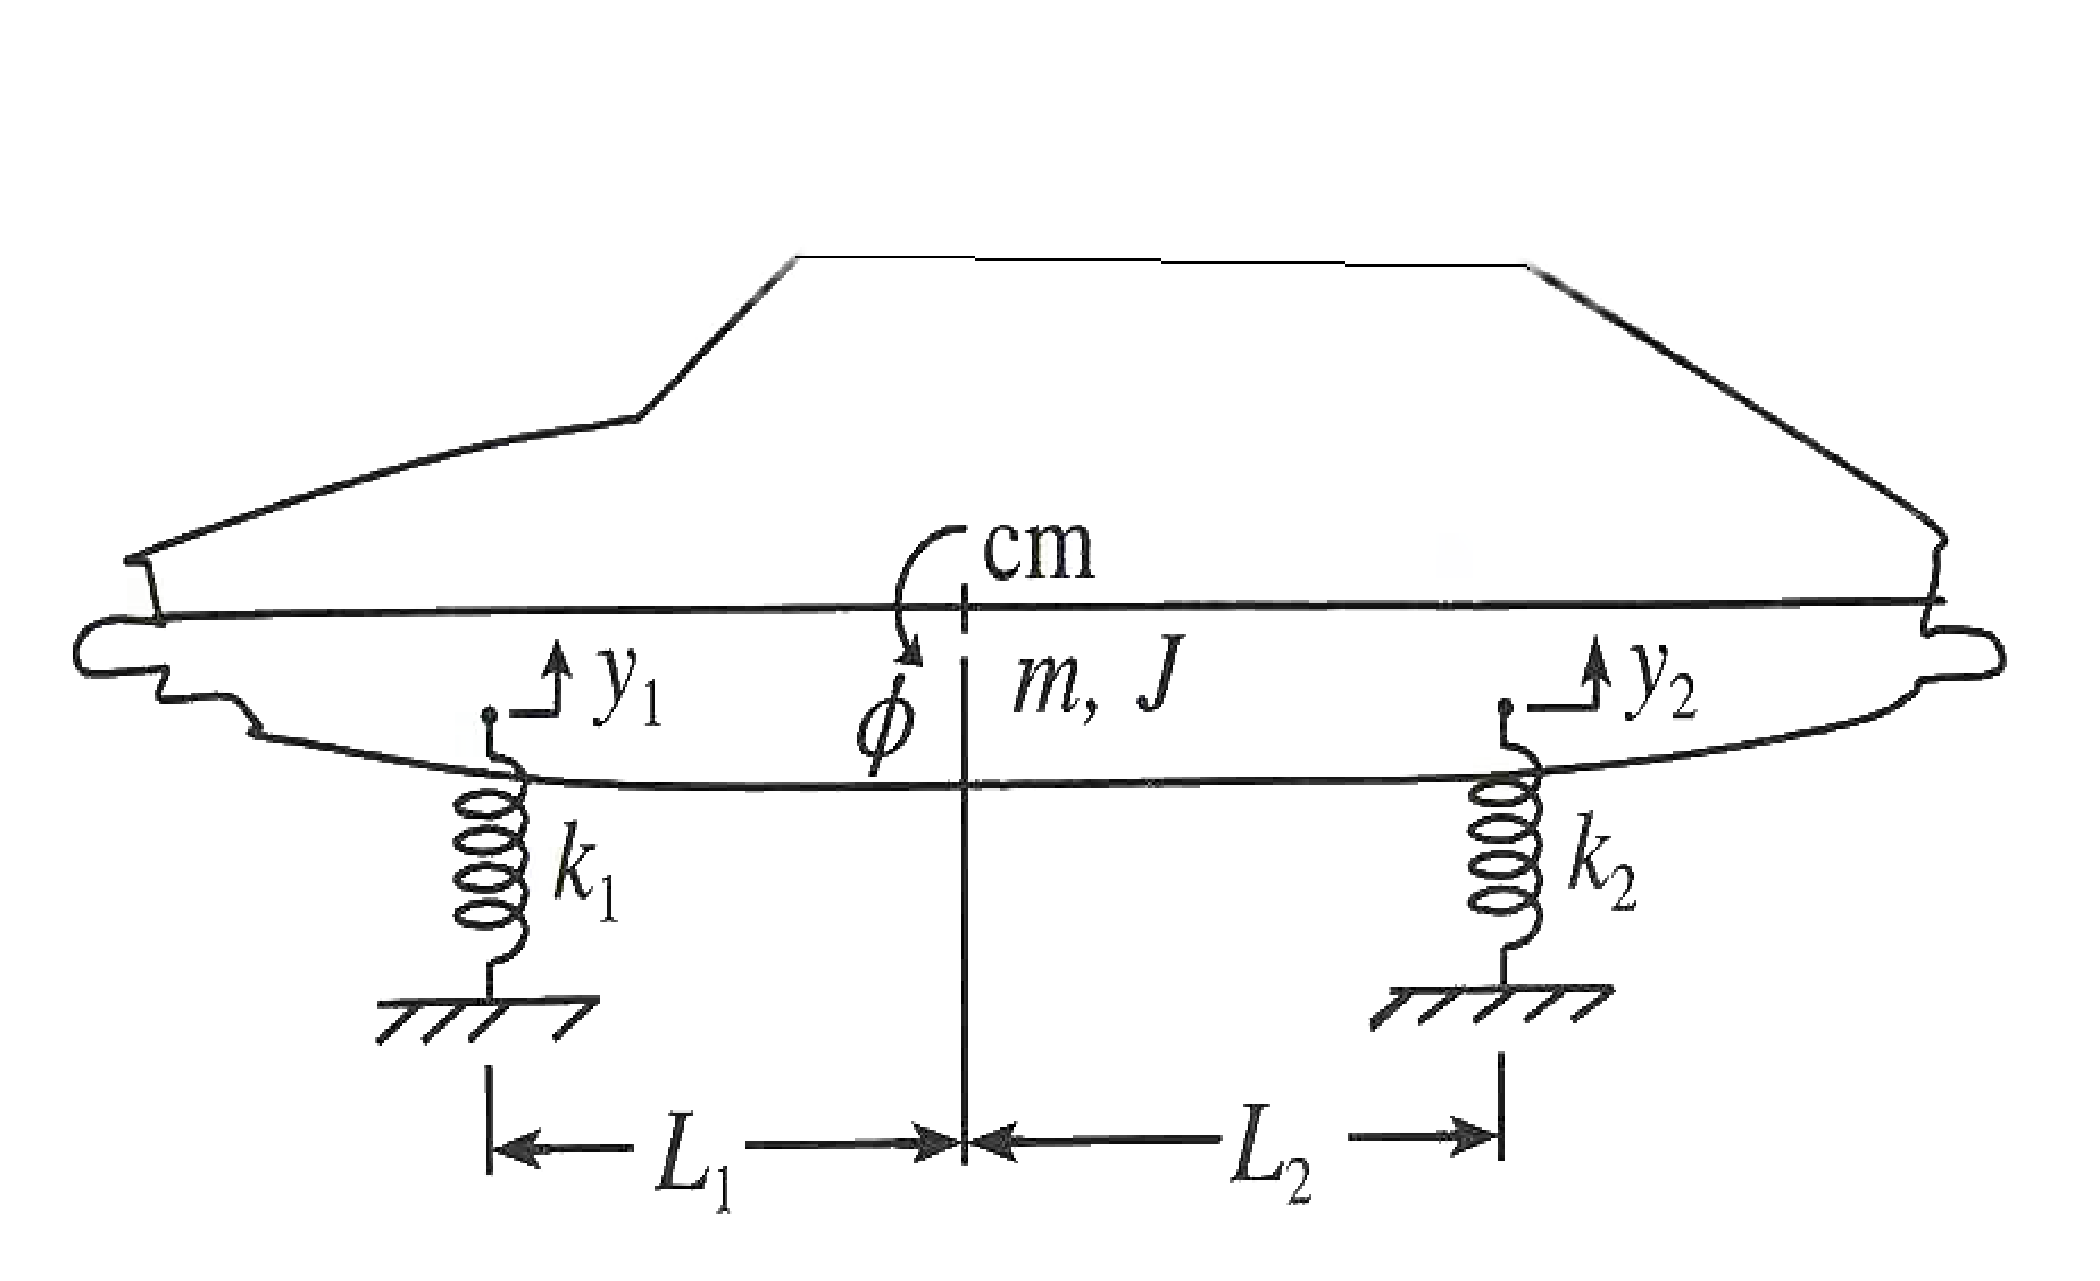
\includegraphics[scale=0.2]{img/may_26_5}
    \end{center}
    \ind The motion of this system is governed by these four coupled
    differential equations. (You don't have to derive them---just
    appreciate that someone has gone through the mechanics for you.)
    \begin{align*}
        \dot{y_1}&=\frac{p_m}{m}-\frac{L_1p_\psi}{J} \\
        \dot{y_2}&=\frac{p_m}{m}+\frac{L_2p_\psi}{J} \\
        \dot{p_m}&=-k_1y_1-k_2y_2-\frac{R_1+R_2}{m}p_m
        -\frac{L_2R_2-L_1R_1}{J}p_{\psi} \\
        \dot{p_\psi}&=L_1k_1y_1-L_2k_2y_2-\frac{L_2R_2-L_1R_1}{m}p_m
        -\frac{L_2^2R_2+L_1^2R_1}{J}p_{\psi}
    \end{align*}
    The four dependent variables are $y_1(t)$ and $y_2(t)$, the
    vertical displacements of the front and rear axles, respectively,
    and $p_m(t)$ and $p_{\psi}(t)$, the linear momentum and angular
    momentum about the mass center of the system, respectively. Here,
    $J$ is the moment of inertia of the car about its center of mass,
    $L_1$ and $L_2$ are the horizontal distances between the front and
    rear axles and the center of mass, $k_1$ and $k_2$ are the spring
    constants, and $R_1$ and $R_2$ are the damping resistance
    constants.\\\\
    \ind Use the following parameter values: $J=mr^2$ with
    $m=1250\text{ kg}$ and $r^2=1.6\text{ m}^2$, $k_1=30\text{
    kN}/\text{m}$, $k_2=32\text{ kN}/\text{m}$, $L_1=1.4\text{ m}$
    and $L_2=1.6\text{ m}$.
    \begin{enumerate}
        \item This is a system of four first-order, linear,
            homogeneous, autonomous differential equations. Write it in
            linear algebra form. Breathe a sign of relief that in this
            entire problem you are not being asked to calculate
            $Pe^{Dt}P^{-1}$ to solve these ODEs.
        \item You already know that the solution to this system of
            ODEs is going to involve terms like $e^{\lambda_1 t}$,
            $e^{\lambda_2 t}$, $e^{\lambda_3 t}$, $e^{\lambda_4 t}$,
            where the $\lambda_i$ are the eigenvalues to the system
            matrix. One common misconception is that $y_1$ involves only
            $e^{\lambda_1 t}$, that $y_2$ involves only $e^{\lambda_2
            t}$, etc.  By imagining how the calculation
            $Pe^{Dt}P^{-1}$ would be performed (but not actually
            performing it), explain why it is more likely that all four
            dependent variables will consist of a linear combination of
            all four exponential terms.
    \end{enumerate}
\end{problem}
\begin{problem}[5 cont.]
    \begin{enumerate}
        \setcounter{enumi}{2}
        \item Suppose that there is no damping in the system
            ($R_1=R_2=0$). Use a technology to help you calculate the
            eigenvalues of the system matrix.  What kind of motion
            (undamped, underdamped, critically damped, or overdamped
            oscillation) characterizes the behavior of the system?  What
            are its vibrational frequencies?  (In other words, if there
            is a term like $\cos(\sigma t)$ in the solution, what is the
            $\sigma$?)  Report these frequencies with the proper units.
        \item Now suppose $R_1=R_2=4000\text{ N s}^2/\text{m}$. What
            kind of motion characterizes the behavior of the system?
        \item Now suppose $R_1=R_2=R$. Find a value of $R$ for which
            the behavior of the system is no longer oscillatory. (You
            don't have to do this in a systematic way. Just picking
            numbers until you find what you need is fine.)
    \end{enumerate}
\end{problem}
\begin{solution}
    \vfill
\end{solution}
\end{document}
